\setlength{\parindent}{4ex}
\setlength{\parskip}{1ex}

\section{User interface design}
In this section are presented or referenced some mockups of the main features and related user interfaces the system is supposed to offer to the user and to the validation service through the proper web-based application.

Mockups show how the user interface is supposed to offer to the user the possibility to interact and make request to the system (obviously such user's interactions will result in a client-server communication of the user/validation service app view with the related server component based on the protocol chosen for that communication).

The main goal of our mockups design process is to build an interface that clearly distinguish functionalities offered by the system taking into account the architectural decoupling offered by the taken design choices.

\subsection{User app}
The user app mockups have been discussed and presented in the User Interfaces section of the \emph{SafeStreets: Requirements Analysis and Specification Document} \cite{RASD}. For further implementation details refer to the \hyperref[sec:implementationChoices]{Implementation Choices} section of this document.

In addition we present the UX diagram to show the flow which the user will follow to navigate inside the application, in accordance with the mockups specified in the RASD:\\

\begin{figure}[ht!]
	\centering
	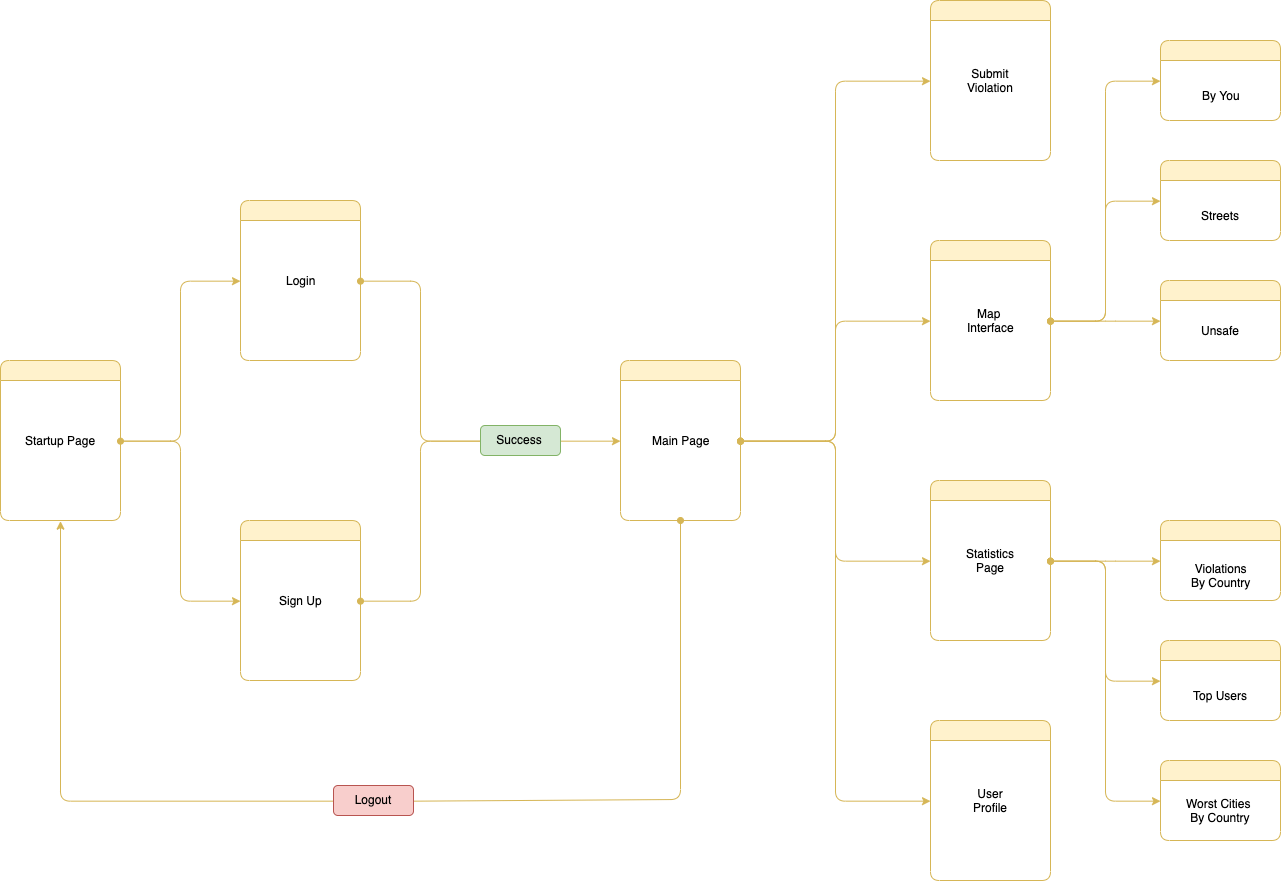
\includegraphics[width=\linewidth]{diagrams/UXdiagram-user.png}
	\caption{
		\label{fig:uxuser} 
		\emph{UX Diagram} - User
	}
\end{figure} 

\subsection{Validation Service app}
The validation service app has a simple interface in order to provide features to validation service operators in a clear and simple way. This interface must be optimised for a desktop monitor size.

The UX diagram presented below shows the flow which the validation operator will follow to navigate in the website, in order to manage the reports submitted.

In accordance to it, the web pages mockups are specified in the following page.\\\\\\

\begin{figure}[ht!]
	\centering
	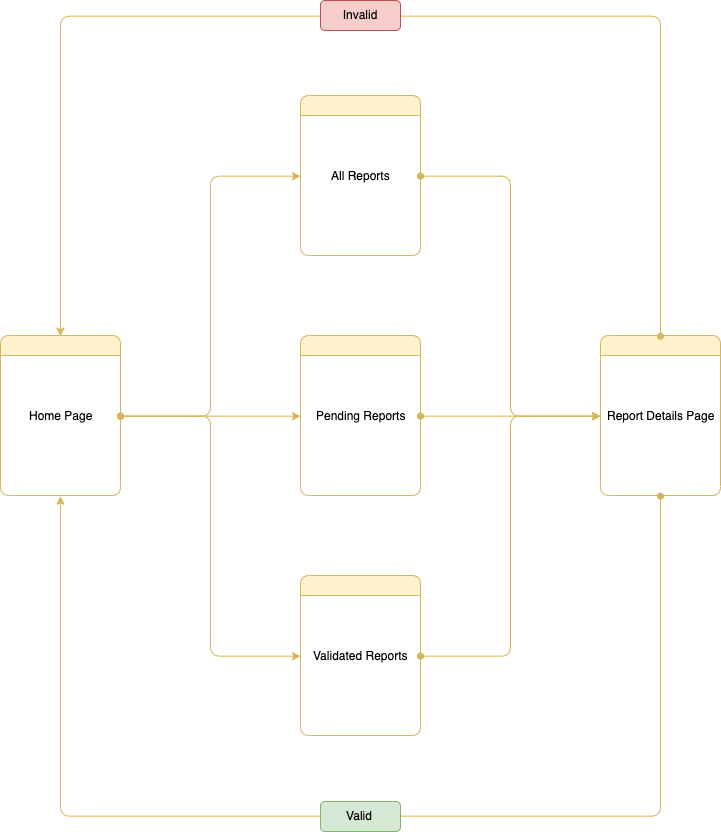
\includegraphics[scale=0.45]{diagrams/UXdiagram-validation.png}
	\caption{
		\label{fig:uxvalidation} 
		\emph{UX Diagram} - Validation Service
	}
\end{figure}

\clearpage
\subsubsection{Home page}
All main features are accessible directly from the home page to provide a rapid and intuitive access to them. \\
From the home page the operator can:
\begin{itemize}
	\item Visualise all the submitted reports
	\item Filter by the pending reports of possibly occurred accidents
	\item Filter by the already validated reports
	\item Delete single or multiple reports
	\item Select a specific report to visualise all the stored data regarding it, accessing the \emph{report details page}\newline\newline
\end{itemize}
 
 \begin{figure}[ht!]
 	\hspace*{-1cm}
			\centering
			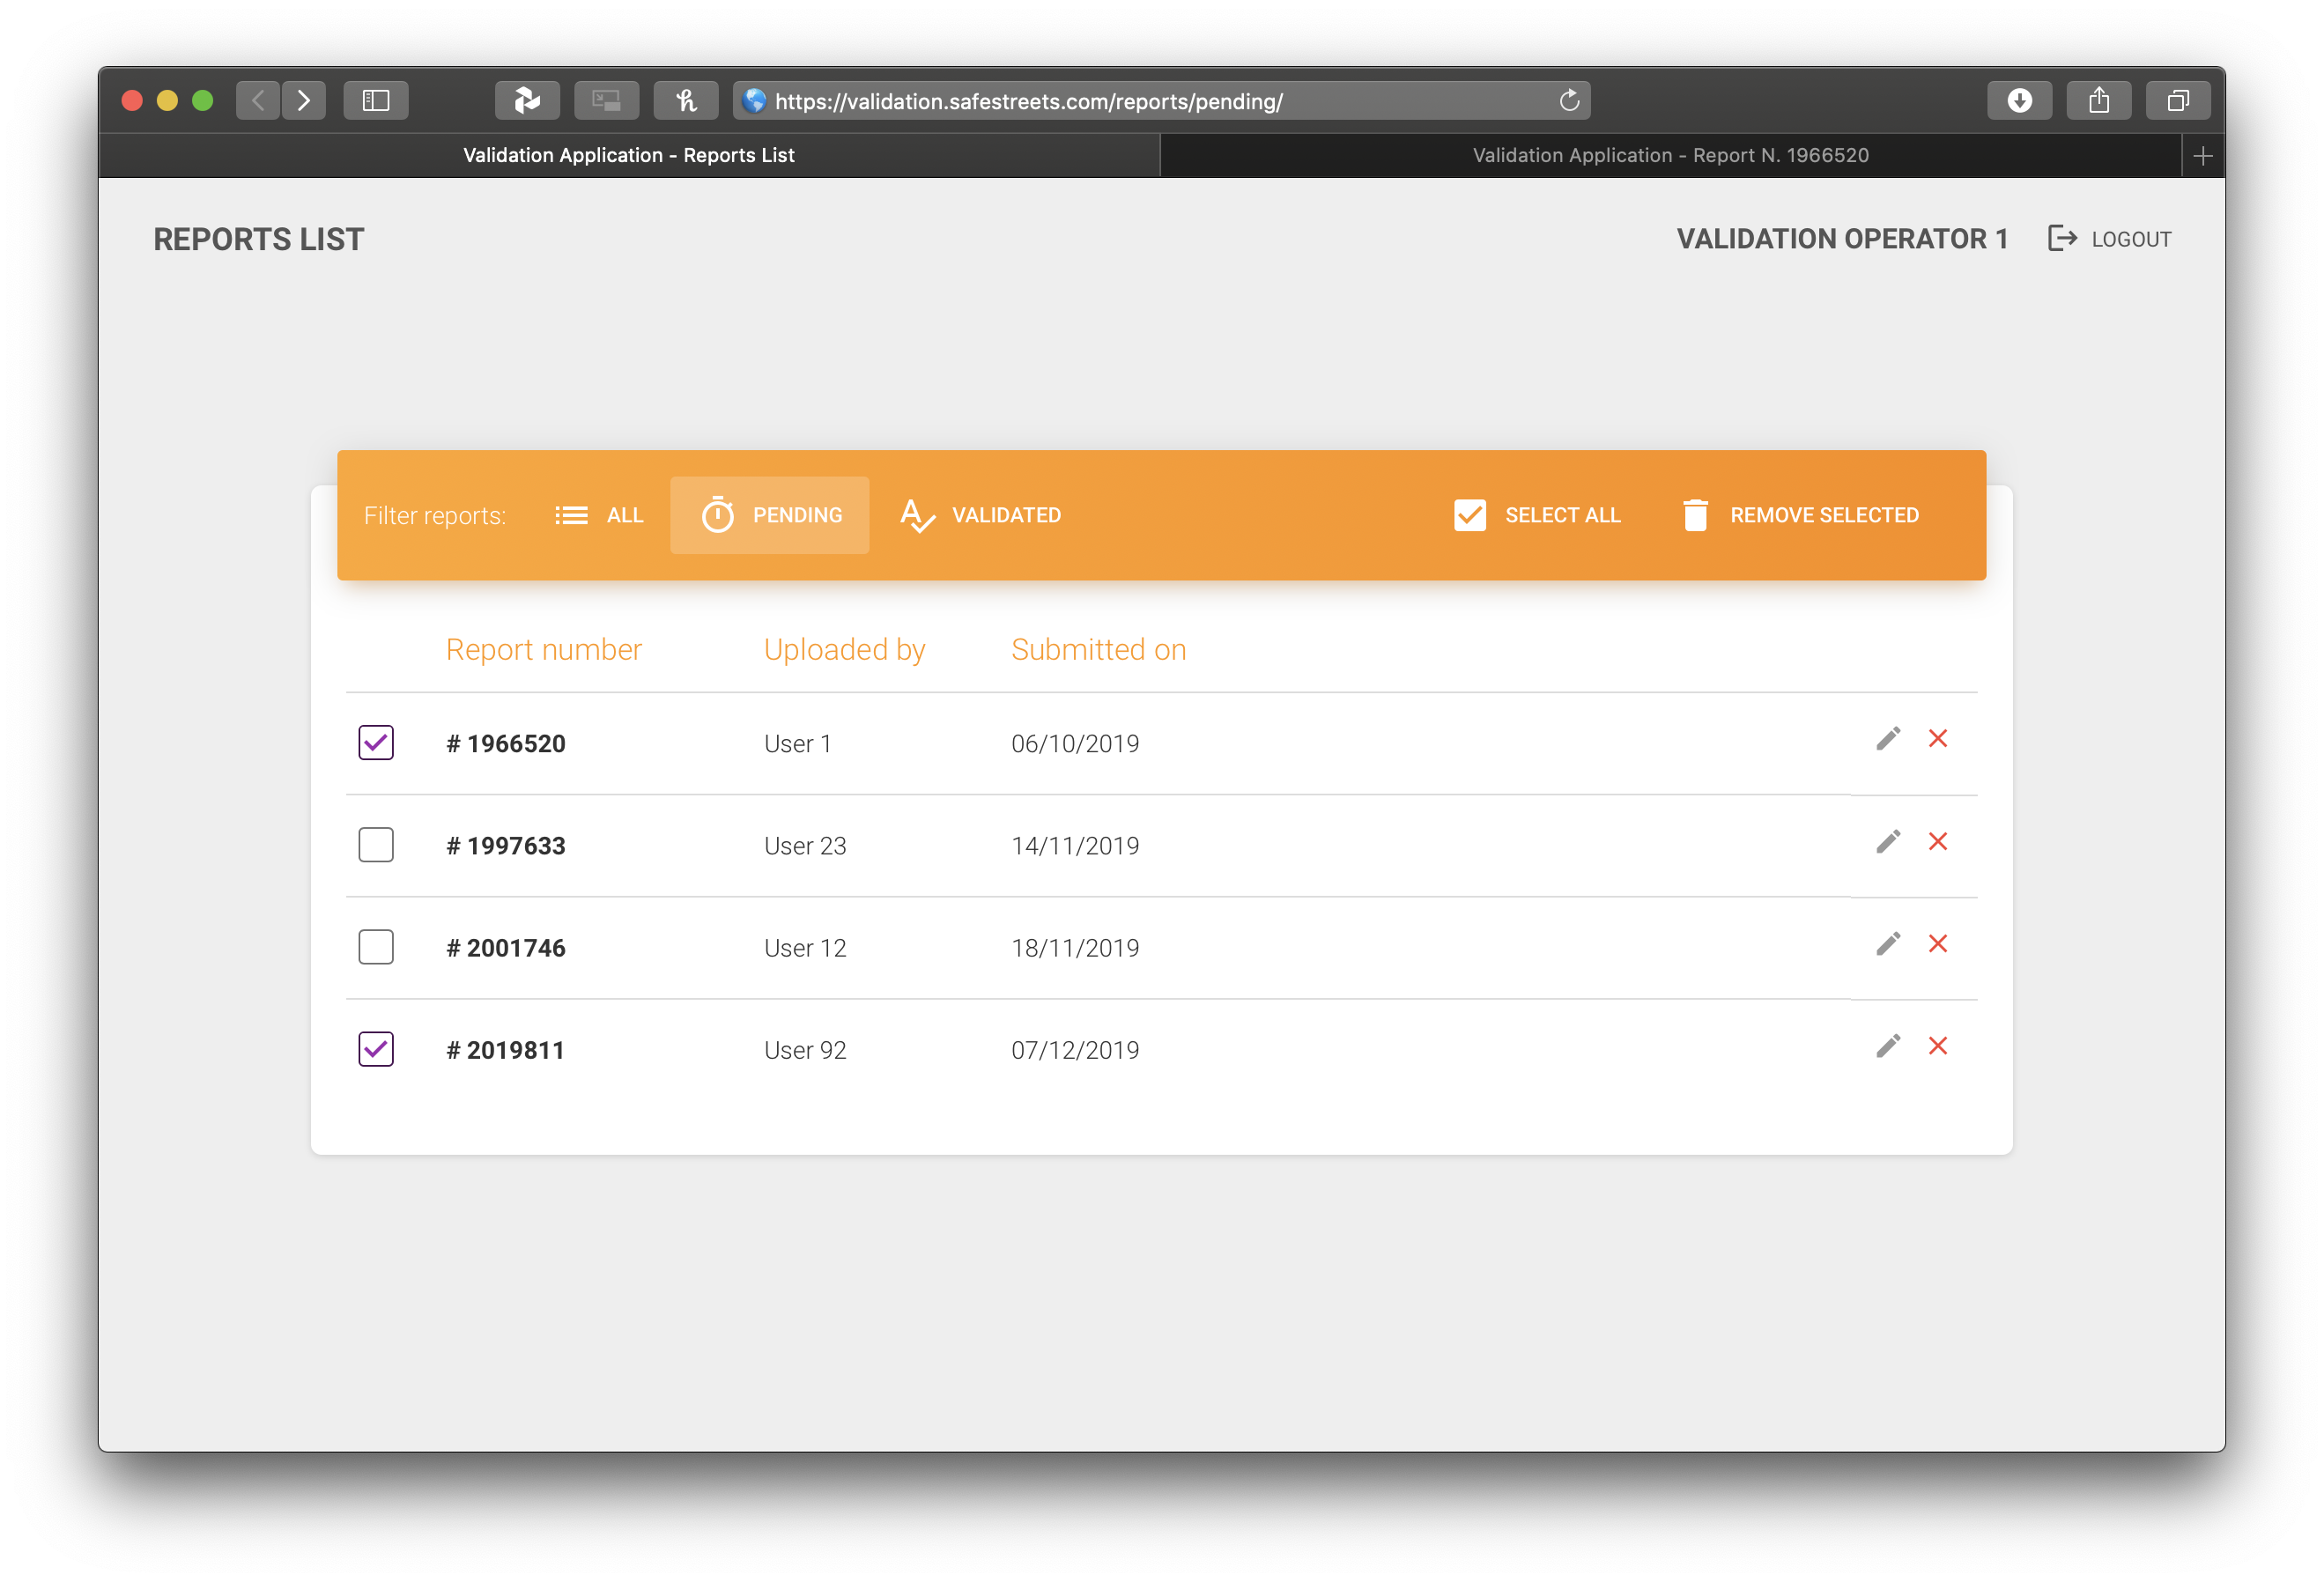
\includegraphics[scale=0.3]{mockups/validationApp1.png}
			\caption{
				\label{fig:cc1} 
				\emph{Validation service home page} mockup
			}
		\end{figure}

		\clearpage
\subsubsection{List of Reports and Violations}

From the report details page, the operator can:
\begin{itemize}
	\item Visualise all the detailed information about the selected report
	\item Visualise the result of the image recognition algorithms associated to the selected report
	\item Manually type the report license plate if not present, wrongly typed by the user, or totally not recognised
	\item Mark and unmark reports as valid in order to transform it into a violation\newline\newline
\end{itemize}

\begin{figure}[ht!]
	\hspace*{-1cm}
	\centering
	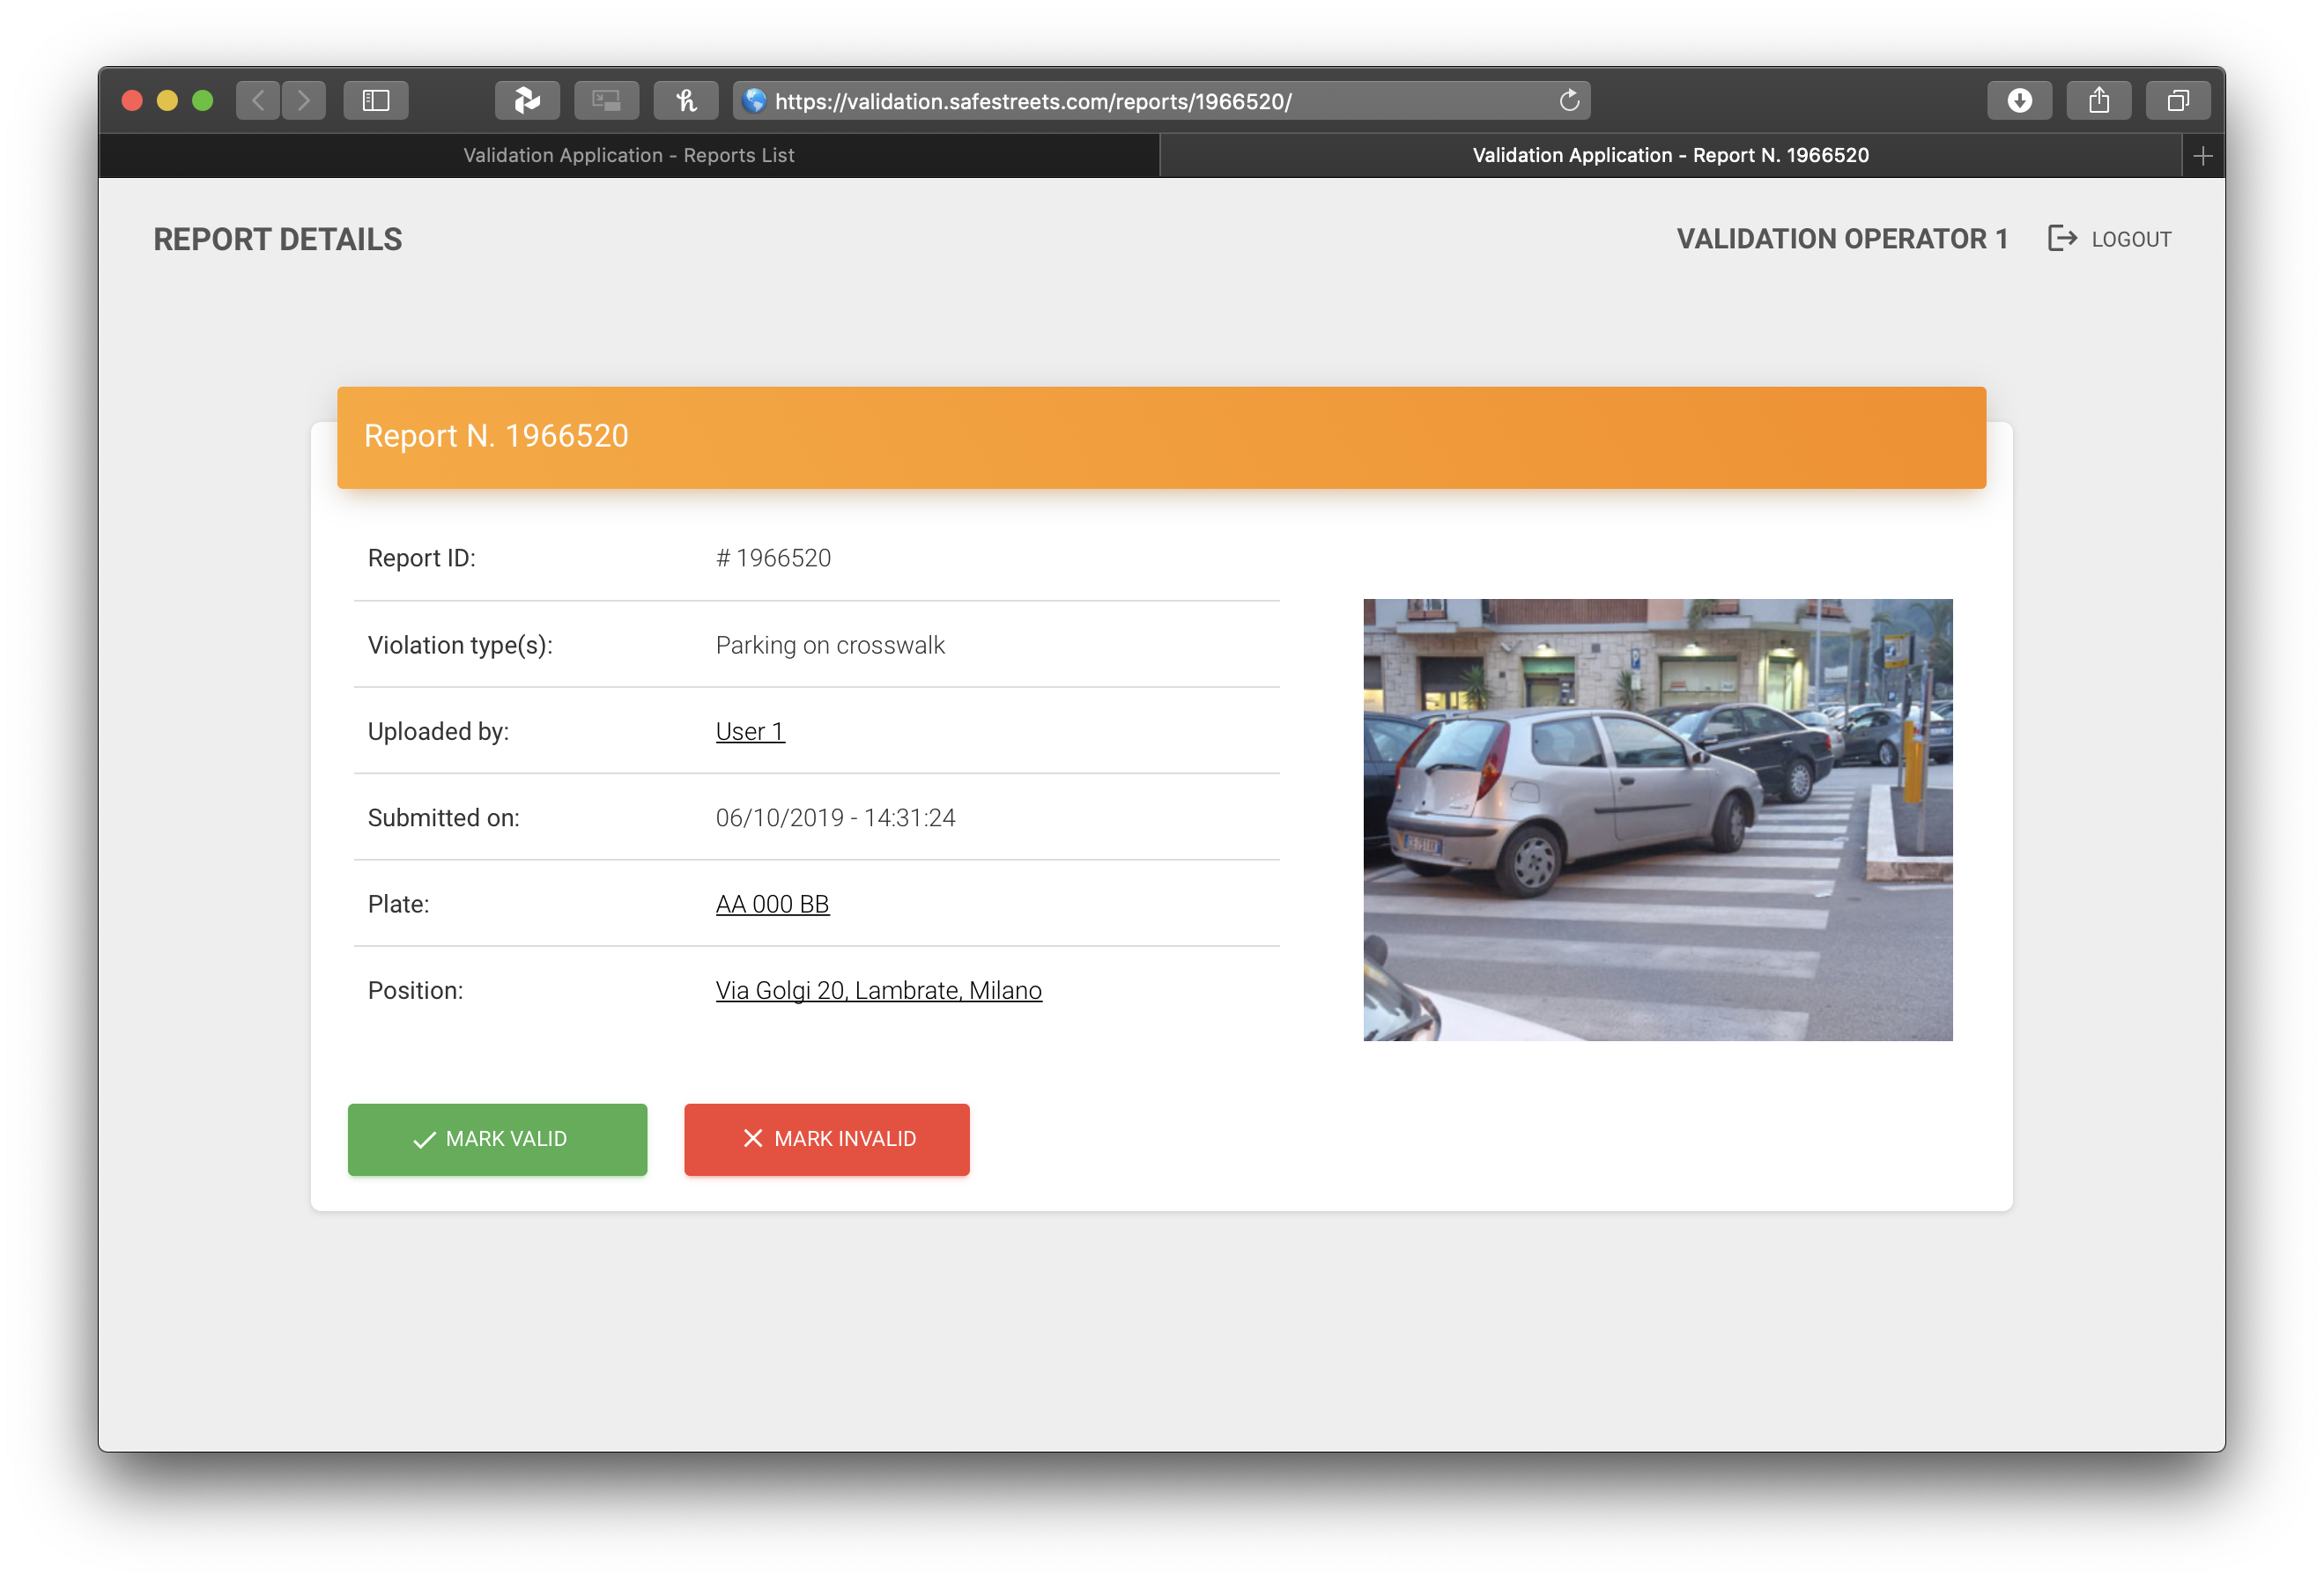
\includegraphics[scale=0.3]{mockups/validationApp2.png}
	\caption{
		\label{fig:cc2} 
		\emph{Validation service reports and violations list} mockup
	}
\end{figure}